\documentclass[11pt,a4paper]{article}
\usepackage{amsmath}
\usepackage{hyperref}
\usepackage{fullpage}
\usepackage{graphicx}

\hypersetup{%
    pdfborder = {0 0 0}
}

\begin{document}

\title{Helios distribution fitting}
\author{David Stansby}
\maketitle

%%%%
\begin{abstract}
A technical summary of the fitting method applied to Helios distribution functions.
\end{abstract}
\section{1D distributions}
The 1D distributions are reduced 3D distributions, which were integrated over all solid angles on board the spacecraft before being transmitted. They are given in the raw files as distribution function\footnote{We are unsure of the units, but know by comparision to the 3D distribution functions that they are dimensions $T/L^{4}$, as a standard 1D reduced distribution function is expected to have.} as a function of speed. The particles were measured in energy per charge ($E/q$) bins, and the speeds calculated assuming all particles were protons; for bin with a retarding potential $V$:
\begin{equation}
	Vq_{p} = \frac{1}{2} m_{p} v^{2}
\end{equation}
\begin{equation}
	v = \sqrt{\frac{2 Vq_{p}}{m_{p}}}
\end{equation}
Particles with a differing $m/q$ ratios will therefore appear at a velocity that is $\sqrt{m/q}$ higher than their true velocity.

\subsection{I1a}
Figure \ref{fig:1D} shows an example of a 1D I1a distribution function.

\subsection{I1b}
Figure \ref{fig:1D} shows an example of a 1D I1b distribution function. Because I1b measured current and not particle counts, a particle with a charge $q$ will contribute a factor $q$ more to I1b compared to I1a. When the proton core of each distribution is normalised to one, a second population at higher velocities lies a factor of 2 higher in I1b, consistent with the population being alpha particles.

\subsection{1D Fits}
\begin{itemize}
	\item If there are no points in (I1a/I3) \textbf{or} I1b no fitting is done (error codes 7 or 8).
\end{itemize}
Points in (I1a/I3) that are greater than the lowest count rate measured are removed. Points in  I1b that are greater than 2 times the lowest count rate measured are removed. This removes points that are at the noise floor.
\begin{itemize}
	\item If there are now no points in (I1a/I3) \textbf{or} I1b no fitting is done (error codes 7 or 8).
	\item If there are now less than 6 points in (I1a/I3) \textbf{or} I1b no fitting is done (error code 5).
\end{itemize}
In order to filter out corrupted distribution functions the following criteria are applied:
\begin{itemize}
	\item I1a
	\begin{itemize}
		\item If the maximum I1b distribution function value is more than 10 times the maximum I1a distribution function value no fitting is done (error code 9)
	\end{itemize}
	\item I3
	\begin{itemize}
		\item If the maximum I3 distribution function value is more than 5 times the maximum I1b distribution function value no fitting is done (error code 9)
	\end{itemize}
\end{itemize}
Initial guesses for the proton core are taken as
\begin{itemize}
	\item $A$: The maximum of (I1a/I3)
	\item $v$: Velocity at maximum value of (I1a/I3)
	\item $v_{th}$: 40 km/s
\end{itemize}

The I1b distribution is then fitted to one Maxwellian:
\begin{equation}
	f \left ( v; n, v_{0}, v_{th} \right ) = n\cdot 4\pi v^{2} \cdot \left (\frac{1}{\pi v_{th}^{2}} \right )^{3/2} e^{-\frac{v - v_{0}}{v_{th}}}
\end{equation}
The fitting is done using least squares minimisation\footnote{\url{https://docs.scipy.org/doc/scipy/reference/generated/scipy.optimize.least_squares.html}} of the residuals calculated from $\left (f_{data} - f_{fit}\right )$ to get best estimates of the 3 parameters. Possible error codes are given in table \ref{tab:1D errors}. The output variables of each individual fit is given in table \ref{tab:1D dict}. If the fitting fails at any stage, all the parameters are set to $nan$ and still saved.

The only fit parameter used for the subsequent 3D fits is the thermal speed.

\section{3D distributions}
The 3D distributions given as distribution function values as a function of $v_{x}$, $v_{y}$, $v_{z}$.
\begin{itemize}
	\item If the 1D fit indicates a corruped I1a distribution (error code 9, table \ref{tab:1D errors}), no 3D fitting is done.
\end{itemize}
Initially the following points are removed from all distribution functions:
\begin{enumerate}
	\item Points with a single count
	\item Points with counts $\geq 32768$
	\item Energy bins 1, 2 and 3 (assumed to consist of only noise)
	\item Points with $\left | \mathbf{v} \right |$ greater than 1,000 times the greatest velocity bin in the 1D I1a distribution
\end{enumerate}

\begin{itemize}
	\item If the distribution now has $\leq 6$ points, no 3D fitting is done (error code 5)
	\item If the distribution now has less than 3 bins resolution in the $\phi$ direction, no 3D fitting is done (error code 12)
	\item If the distribution now has less than 3 bins resolution in the $\theta$ direction, no 3D fitting is done (error code 12)
	\item If the minimum $\left | \mathbf{v} \right |$ is greater than the velocity at which the I1a 1D distribution is a maximum, no 3D fitting is done (error code 10)
\end{itemize}

A check is then done for magnetic field data availability. If 4Hz data is available when the distribution was measured, that is used. Otherwise if 6s data is available that is used. An average ($\mathbf{B}_{0}$)\footnote{For Helios 2 the $B_y$ and $B_z$ 4Hz components are flipped to agree with the 6s magnetic field data} and standard deviation of each component taken. The velocities are then rotated into the frame aligned with $\mathbf{B}_{0}$. If no magnetic field data is present, fitting is done in the original spacecraft frame and only the bulk velocity parameters saved.

A 3D bi-Maxwellian fit is done of the following form (fit parameters in bold):
\begin{equation}
	f \left ( v_{\parallel}, v_{\perp 1}, v_{\perp 2} \right ) = \mathbf{A} \cdot \exp - \left \{ \left ( \frac{v_{\parallel} - \mathbf{u}_{\parallel}}{\mathbf{w}_{\parallel}} \right )^{2} + \left ( \frac{v_{\perp 1} - \mathbf{u}_{\perp 1}}{\mathbf{w}_{\perp}} \right )^{2} + \left ( \frac{v_{\perp 2} - \mathbf{u}_{\perp 2}}{\mathbf{w}_{\perp}} \right )^{2} \right \}
\end{equation}
The 6 fit parameters are amplitude ($A$), 3 velocities ($u_{\parallel}$, $u_{\perp 1}$, $u_{\perp 2}$), and 2 thermal speeds ($w_{\perp}$, $w_{\parallel}$). Initial guesses for these parameters are given in table \ref{tab:3D param guesses}.

The fit is done using least squares minimisation\footnote{\url{https://docs.scipy.org/doc/scipy/reference/generated/scipy.optimize.least_squares.html}} of the residuals calculated from $\left (f_{data} - f_{fit}\right )$.
\begin{itemize}
	\item If the least squares fitting function doesn't return a success status code, results are ignored (error code 6)
	\item If the amplitude returned is greater than 10 times the maximum value of the distribution function, it is physically unrealistic and results are ignored (error code 11)
	\item If the amplitude returned is less than 0.1 times the maximum value of the distribution function, it is physically unrealistic and results are ignored (error code 11)
	\item If the amplitude returned is negative, results are ignored (error code 11)
	\item If the bulk velocity is outside the 3D array of velocities where the distribution function was measured, results are ignored (error code 4)
\end{itemize}
The number density is calculated using
\begin{equation}
	n = A \cdot \pi^{3/2}w_{\perp}w_{\perp}w_{\parallel}
\end{equation}
and temperatures calculated using
\begin{equation}
	T_{\perp / \parallel} = \frac{m_{p}w_{\perp / \parallel}^{2}}{2k_{B}}
\end{equation}
Possible error codes are given in table \ref{tab:3D errors}.

The output dictionary of each individual fit is given in table \ref{tab:3D dict}. If the fitting fails at any stage, all the parameters are set to $nan$ and still saved. In addition to the fitted parameters, some orbital data from the merged data files is added to the output.

Figure \ref{fig:3D} shows an example of 3D distributions and fitting. The bottom panel illustrates that the fitting method is not sensitive to the beam population.

\section{Caveats}

\appendix
%%%%%%%%
\section{Tables and figures}
\begin{table}[h]
	\centering
	\begin{tabular}{| c | c | c | }
		\hline
		Code &	Explanation 						& \% points\\ \hline \hline
		1 &		Fitting successful					& 86.1 \\ \hline
		5 &		Less than 6 points available for fitting	& 12.9\\ \hline
		7 &		No non-noise I1a data available		& 0.19\\ \hline
		8 & 		No non-noise I1b data available		& 0.14\\ \hline
		9 &		Distribution file is corrupted		& 0.18\\ \hline
	\end{tabular}
	\caption{Possible error codes returned by 1D fitting process. Percentage points are for Helios 2 entire mission, with total number of distributions = 892,905.}
	\label{tab:1D errors}
\end{table}

\begin{table}
	\centering
	\begin{tabular}{| c | c | c |}
		\hline
		Parameter 			& Parameter name	& Units 			\\ \hline \hline \hline
		Proton number density 	& n\_p			& $cm^{-3}$		\\ \hline
		Proton velocity		 	& v\_p			& $km\cdot s^{-1}$	\\ \hline
		Proton thermal speed 	& vth\_p			& $km\cdot s^{-1}$	\\ \hline
		Proton temperature	 	& T\_p			& Kelvin			\\ \hline \hline
		Time				 	& Time			& 				\\ \hline
		Fitting status		 	& status			& 				\\ \hline
		Instrument		 	& Instrument		& 				\\ \hline
	\end{tabular}
	\caption{Variables output by the 1D fitting process}
	\label{tab:1D dict}
\end{table}

\begin{table}
	\centering
	\begin{tabular}{| c | c | c |}
		\hline
		Parameter 		& Initial guess 1								& Initial guess 2	\\ \hline  \hline
		Amplitude		& Maximum 3D distribution function value			&				\\ \hline
		Bulk velocity	 	& Numerical moment from whole 3D distribution function	& 	\\ \hline
		Thermal speeds 	& 1D thermal speed fit value							& 40 km/s	\\ \hline
	\end{tabular}
	\caption{Initial guesses for the 3D fit parameters}
	\label{tab:3D param guesses}
\end{table}

\begin{table}
	\centering
	\begin{tabular}{| c | c |  c |}
		\hline
		Code &	Explanation 							& \% points	\\ \hline \hline
		1 &		Fitting successful						& 65.6		\\ \hline
		2 &		No magnetic field data available 			& 30.4		\\ \hline
		4 &		Fitted velocity outside measurement array	& 0.33		 \\ \hline
		5 &		Less than 6 points available for fitting		& 0.40		 \\ \hline
		9 &		Distribution file is corrupted 			& 0.18		\\ \hline
		10&		1D proton peak not present in 3D distribution	& 1.39	 \\ \hline
		11&		Number density physically unrealistic 		& 0.88		\\ \hline
		12&		Less than 3 angular bins present in either direction	& 0.69	 \\ \hline
	\end{tabular}
	\caption{Possible error codes returned by 3D fitting process. Percentage points are for Helios 2 entire mission, with total number of distributions = 892,905.}
	\label{tab:3D errors}
\end{table}

\begin{table}[h]
	\centering
	\begin{tabular}{| c | c | c |}
		\hline
		Parameter 					& Parameter label	& Units 				\\ \hline \hline \hline
		Proton number density 			& n\_p			& $cm^{-3}$			\\ \hline
		Proton $x$ velocity		 		& vp\_x			& $km\cdot s^{-1}$	\\ \hline
		Proton $y$ velocity		 		& vp\_y			& $km\cdot s^{-1}$	\\ \hline
		Proton $z$ velocity		 		& vp\_z			& $km\cdot s^{-1}$	\\ \hline
		Proton perpendicular thermal speed 	& vth\_p\_perp		& $km\cdot s^{-1}$	\\ \hline
		Proton parallel thermal speed 		& vth\_p\_par		& $km\cdot s^{-1}$	\\ \hline
		Proton perpendicular temperature	& Tp\_perp		& Kelvin				\\ \hline
		Proton parallel temperature	 	& Tp\_par			& Kelvin				\\ \hline \hline
		$B_{x}$						& Bx				& nT					\\ \hline
		$B_{y}$						& By				& nT					\\ \hline
		$B_{z}$						& Bz				& nT					\\ \hline
		Magnetic field standard deviation	& sigma B			& nT					\\ \hline \hline
		Time						 	& Time			& 					\\ \hline
		Fitting status					& status			& 					\\ \hline
		Instrument		 			& Instrument		& 					\\ \hline
		Magnetic field instrument			& B instrument		&				\\ \hline \hline
		Sun-spacecraft distance			& r\_sun			& AU				\\ \hline
		Carrington longitude				& clong			& Degrees			\\ \hline
		Carrington lattitude				& clat			& Degrees			\\ \hline
		Carrinton rotation number			& carrot			&					\\ \hline
		Spacecraft-Earth angle			& earth\_he\_angle	& Degrees			\\ \hline

	\end{tabular}
	\caption{Final data output. The top set of values are the fitted parameters, the middle set give information on the fit, and the bottom set are Helios orbital parameters.}
	\label{tab:3D dict}
\end{table}

\begin{figure}[h]
	\centering
	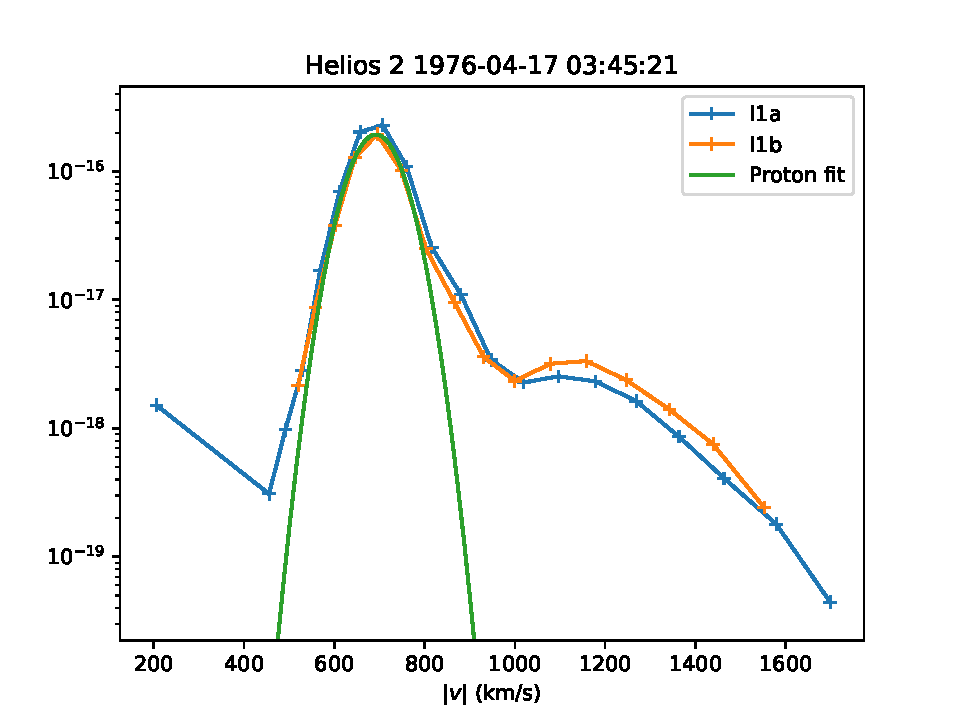
\includegraphics[width=1\textwidth]{1D_example}
	\caption{1D distribution function examples. Blue line shows I1a distribution function and orange line shows I1b distribution for the same interval. Green line shows the result of 1D Maxwellian fitting.}
	\label{fig:1D}
\end{figure}

\begin{figure}[h]
	\centering
	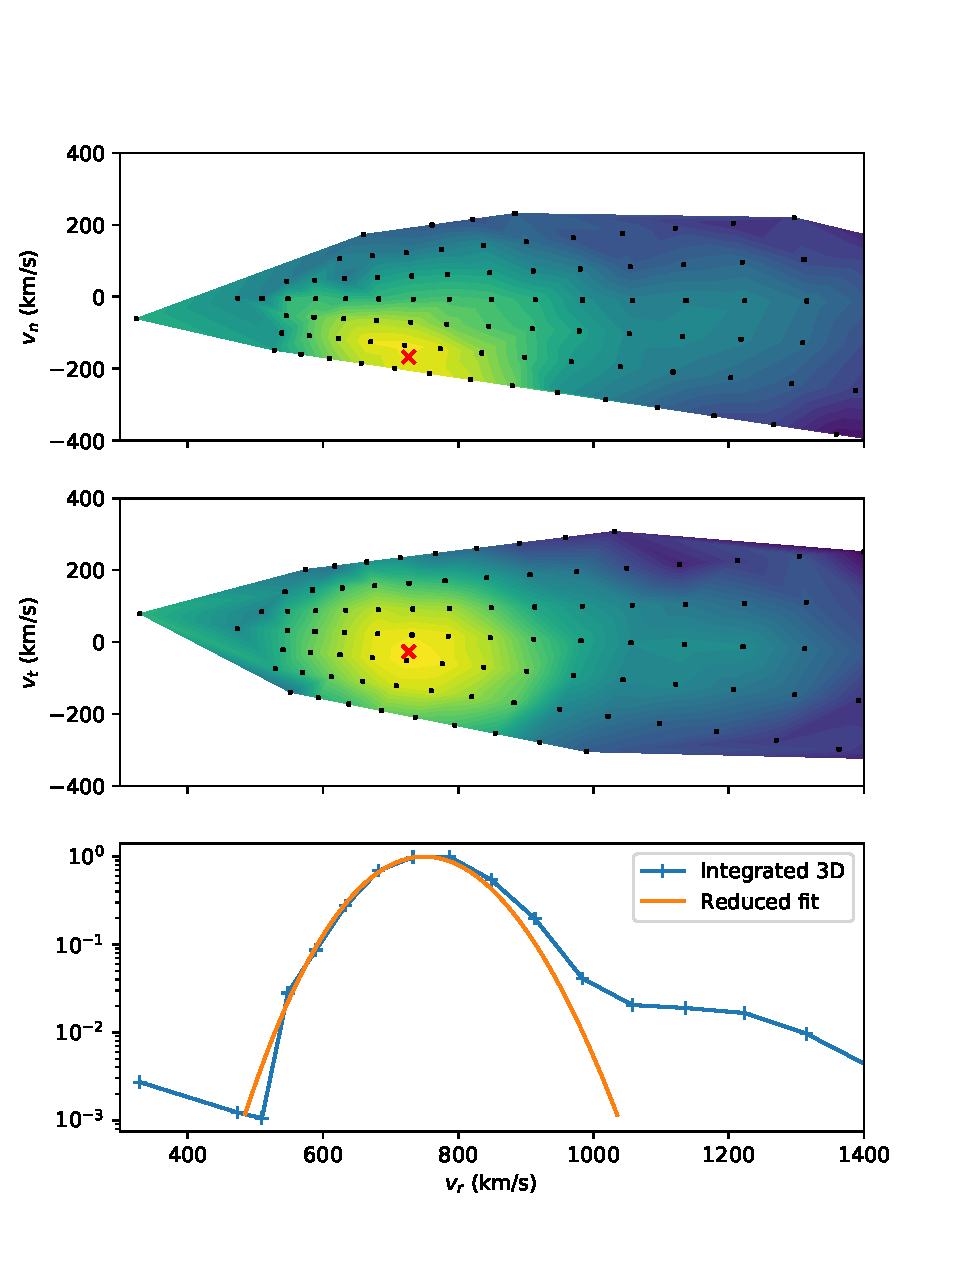
\includegraphics[width=1\textwidth]{3D_example}
	\caption{Top panel shows reduced 2D distribution function in the R-N plane in a RTN co-ordinate system. Middle panel shows reduced 2D distribution function in the R-T plane. Red crosses denote the bulk velocity of the fitted bi-Maxwellian. Bottom panel shows reduced 1D distribution function in blue, and the fitted bi-Maxwellian numerically reduced to 1D in orange.}
	\label{fig:3D}
\end{figure}

\end{document}